\documentclass{amsart}

\usepackage{graphicx}

\title{Homework 4}
\author{James Lee\\
\texttt{jameslee@gwu.edu}}

\begin{document}
\maketitle

\section{Exploiting the S-box}
The first step in breaking the cipher described in the assignment was to exploit the S-box to determine its linear properties.  I noted that, despite being presented as an eight bit S-box in the assignment, the left and right four bits of input and output were completely independent, so I treated it like a four bit S-box.

I modified the code that I used to exploit the S-box in homework three to find the biases of all input and output masks:

\begin{quote}
\begin{verbatim}
% ./sbox-lapprox 
------------------------
| No|IMask|OMask|  Bias|
------------------------
|  1|    0|    0| 0.500|
|  2|    7|    3|-0.375|
|  3|    1|    6|-0.375|
|  4|    F|    D| 0.250|
|  5|    F|    5| 0.250|
|  6|    E|    B|-0.250|
|  7|    E|    7|-0.250|
...
\end{verbatim}
\end{quote}

This helped me draw a linear approximation between plaintext bits and ciphertext bits with a high bias in the next step.

\section{Generating a Linear Approximation}
Because the P-box only shifts bits by the width of the S-box, there is no ``fanning out'' of bits as they propagate through the SPN.  This made it simpler to choose approximations.  I just had to select input and output masks of S-boxes that would give me a high bias.  My choice can be seen graphically in Figure \ref{fig:spn}.  For the first four bits of input and output, the approximation is:
\begin{align*}
P_{12}\oplus K_{112} &= V_{114}\oplus V_{113}&\textrm{with bias } \epsilon_1=-0.375\\
V_{114}\oplus V_{113}\oplus K_{210}\oplus K_{29} &= V_{211}\oplus V_{29}\oplus V_{28}&\textrm{with bias } \epsilon_2=0.250\\
V_{211}\oplus V_{29}\oplus V_{28}\oplus &&\\
K_{37}\oplus K_{35}\oplus K_{34} &= V_{37}\oplus V_{36}\oplus V_{35}&\textrm{with bias } \epsilon_3=0.250\\
\end{align*}

Adding in the fourth round subkey bits gives us an approximation of the bits right before the last S-box:
\[
V_{37}\oplus V_{36}\oplus V_{35}\oplus K_{43}\oplus K_{42}\oplus K_{41} = U_{43}\oplus U_{422}\oplus U_{421}
\]
all of which simplifies to:
\[
P_{12}\oplus U_{43}\oplus U_{42}\oplus U_{41}\oplus\Sigma_K = 0
\]
where
\[
\Sigma_K = K_{112} \oplus K_{210} \oplus K_{29} \oplus K_{37}\oplus K_{35}\oplus K_{34}\oplus K_{43}\oplus K_{42}\oplus K_{41}
\]
with bias $\epsilon_{1,2,3}=2^2(-0.375)(0.250)(0.250)=-0.09375$ by the piling-up lemma (or 0.09375 depending on whether $\Sigma_K$ is 0 or 1).

\begin{figure}[h]
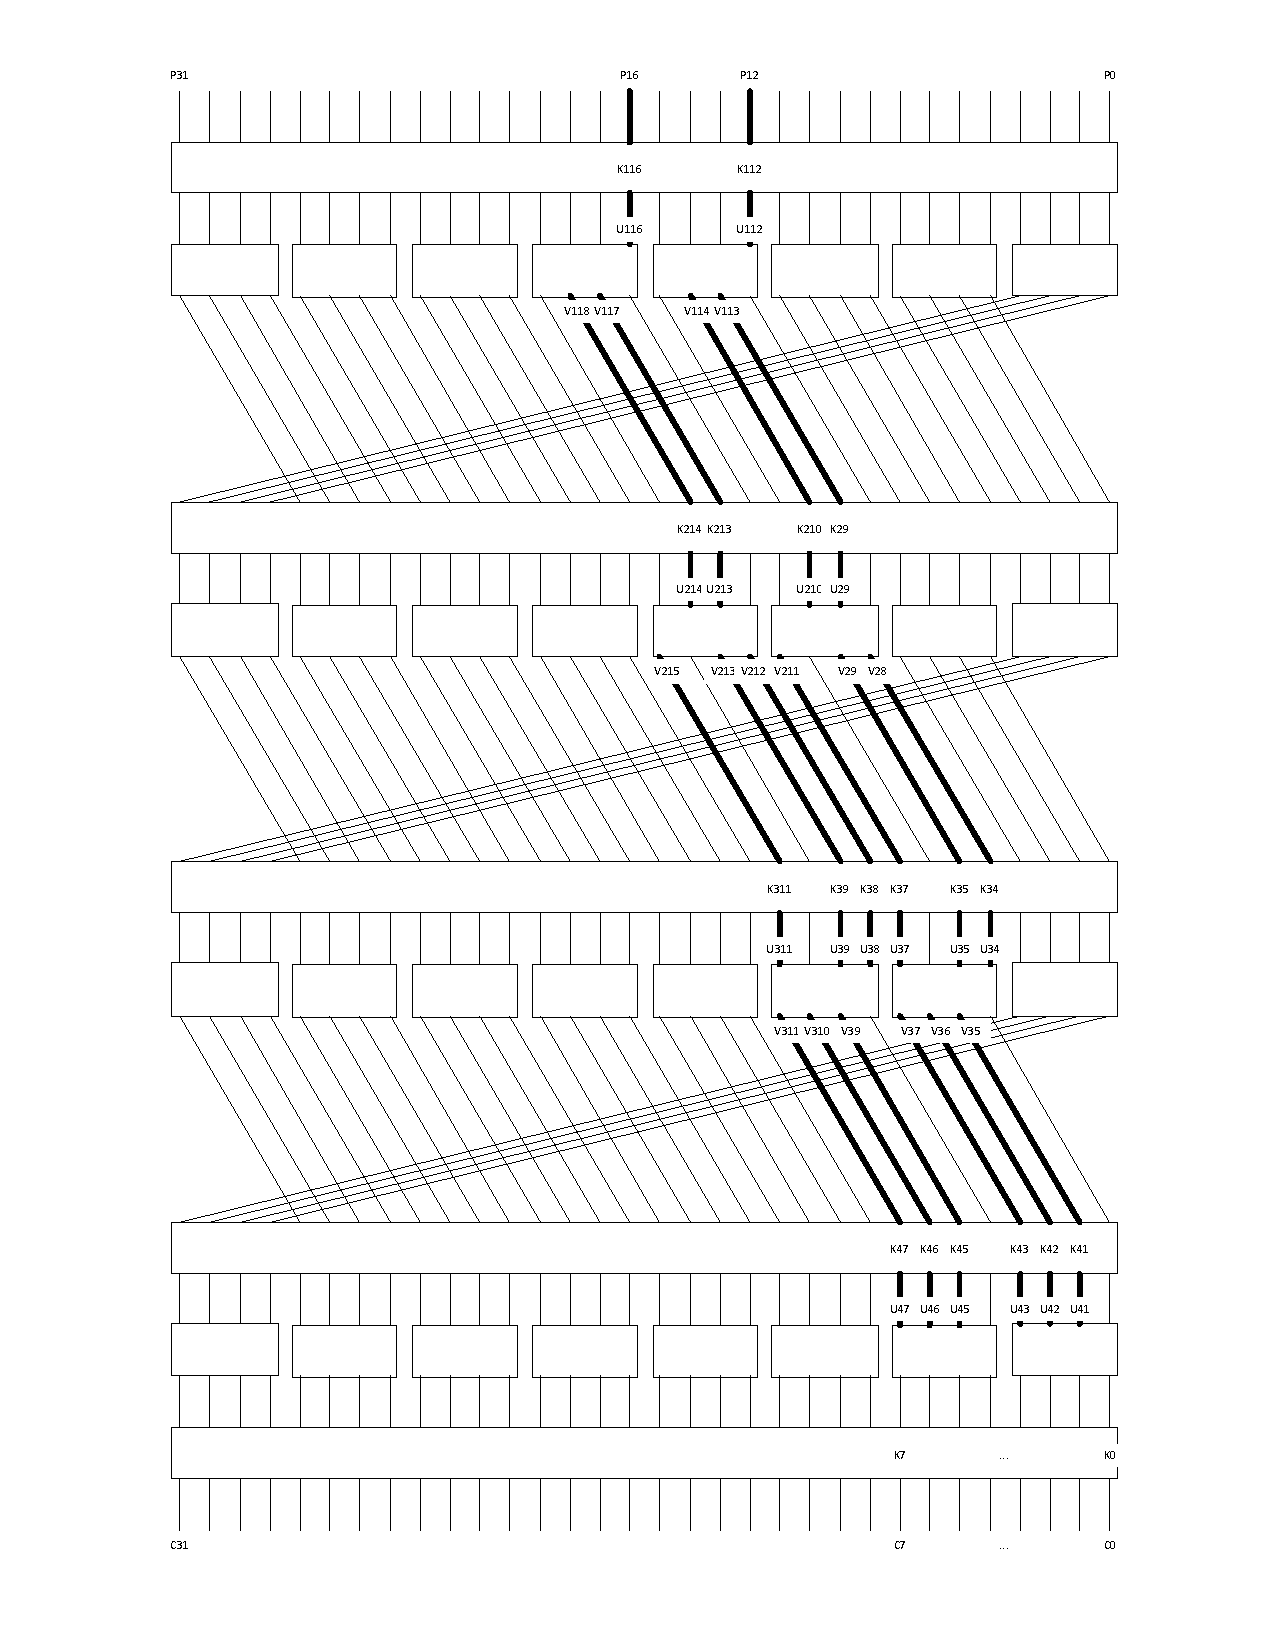
\includegraphics[width=.9\textwidth]{spn.pdf}
\caption{A graphical representation of the SPN with my selected approximation in bold.}
\label{fig:spn}
\end{figure}

\section{Generating Plaintext-Ciphertext Pairs}
The next step in breaking the cipher was to generate enough plaintext-ciphertext pairs to have a reasonable chance of guessing the right key.  According to Matsui, I would need to generate on the order of $\epsilon^{-2}=(0.09375)^{-2}\approx 114$ pairs using the approximation I chose.  But considering that more pairs couldn't hurt, and it is fast to iterate over all possible four bit keys for every pair, I chose to generate 5000.

I do this step in \texttt{generate-pc-pairs.cpp}, modified from code from homework two.  I am careful to generate valid pairs from a random key, decrypting every generated ciphertext to test whether it matches the original random plaintext, before outputting it.

Running the program prints out the key bits $K_7\ldots K_0$ for checking whether the next step guesses the right key bits:

\begin{quote}
\begin{verbatim}
% gmake pc-pairs.txt
./generate-pc-pairs
Try to guess these key bits: 1101 1010
\end{verbatim}
\end{quote}

\section{Extracting The Key Bits}
To extract the key bits, in \texttt{cryptanalyze.cpp} I read each of the 5000 plaintext-ciphertext pairs, and for each one I try all possible four bit keys (twice, one for the left track, one for the right track).  I XOR each key with the corresponding ciphertext bits, and run it backwards through the last round S-box.  This gives me the bits $U_{43}$, $U_{42}$, and $U_{41}$ (or $U_{47}$, $U_{46}$, and $U_{45}$) which I can then XOR all together with $P_{12}$ (or $P_{16}$) and test whether the result equals 0.  Theoretically, a perfect cipher would have the bits equal 0 exactly 50\% of the time.  But, with the approximation I chose, I should see a devation of about 9\% (0.09375) less or more than 50\% for the correctly chosen key.

Running the code shows that my selected approximation extracts the correct key bits, most of the time:

\begin{quote}
\begin{verbatim}
% rm pc-pairs.txt; gmake run
./generate-pc-pairs
Try to guess these key bits: 1110 1011 
./cryptanalyze
Top 16 keys:
Key1  Count1  Key2  Count2
--------------------------
1101    1267  1011    1267
0010    1258  1001    1258
1110    1254  0111    1254
1100    1237  1000    1237
0001     651  0101     651
1111     636  0001     636
...
\end{verbatim}
\end{quote}

The ``count'' is the absolute value of the number of times the equation holds minus half the number of plaintext-ciphertext pairs.  The correct key is usually in the top four of the 16 possible keys.

Unfortunately, I had to relax the problem in order to get this result.  I had to eliminate all but the last round key when generating the plaintext-ciphertext pairs.  With a random key for each of the five rounds, I was unable to reliably extract any of the last round key bits.  I tried solving the issue many ways with no success:

\begin{enumerate}
\item To validate my implementation, I performed the same steps on the S-box presented in Heys' paper.  To my suprised it worked the first time and every time.  This implementation is the \texttt{heys} subdirectory of my submission:
\begin{quote}
\begin{verbatim}
% gmake -C heys 
gmake: Entering directory `/nest/home/school/CSCI6331/hw4/heys'
<compiling>
./generate-pc-pairs
Try to guess these key bits: 0101 0011 
./cryptanalyze
0101 0011 4586
0101 1111 5363
1000 0011 5319
1000 1110 4693
...
\end{verbatim}
\end{quote}

\item Thinking my linear approximation might be weak, or not ideal, I tried about a dozen others.

\item I tried aggregating the results of several combinations.

\item I tried increasing the number of plaintext-ciphertext pairs all the way up to 100,000.

\item Since the P-box for the assignment's SPN does not play any role, I tried finding the ideal linear approximation by reimplementing \texttt{cryptanalyze.cpp} in \texttt{find-best-approx.cpp}.  In this implementation, I let the algorithm know what the right key bits are, then let it try all possible input and output masks over a set of 5000 plaintext-ciphertext pairs.  The input and output mask which extracts the right key bits with the highest bias is outputted:
\begin{quote}
\begin{verbatim}
% ./generate-pc-pairs
Try to guess these key bits: 1000 1101 
% gmake find-best-approx && ./find-best-approx 1101
Found key 13 with approx (2, 4) and bias 1890
\end{verbatim}
\end{quote}
Unfortunately, the algorithm would output a different pair of masks for each set of plaintext-ciphertext pairs presented to it, so it did not reveal any patterns to me.
\end{enumerate}

I would have liked to have gotten the key bits without having to relax the problem, but even thinking like an adversary would, nothing I tried seemed to help.  In the end, I do at least feel like I understand linear cryptanalysis better.
\end{document}
